% main.tex
\documentclass[11pt]{article}

\usepackage[letterpaper, margin=1in]{geometry}
\usepackage{setspace}
\usepackage[round]{natbib}
\usepackage{graphicx}
\graphicspath{{../figs/}}
\usepackage{caption}
\usepackage{subcaption}
\usepackage{threeparttable}
\usepackage{hyperref}
\usepackage{xcolor}
\usepackage{amsmath}
\usepackage{amssymb}
\usepackage{bm}
\usepackage{float}
\usepackage{amsthm}
\usepackage{booktabs}
\usepackage{tabularx}
\usepackage{siunitx}
\usepackage{tikz}
\usetikzlibrary{positioning, arrows.meta, shapes.geometric}

\doublespacing

\hypersetup{
    colorlinks=true,
    linkcolor={red!50!black},
    citecolor={blue!50!black},
    urlcolor={blue!80!black}
}

\title{Big Effects from Small Samples:\\
Album Releases and Traffic Fatalities}

\author{
Gaurav Sood\thanks{\href{mailto:gsood07@gmail.com}{\texttt{gsood07@gmail.com}}}
\and
Daniel Weitzel\thanks{\href{mailto:weitzeld@ceu.edu}{\texttt{weitzeld@ceu.edu}}}
}

\date{\today\thanks{First version April 12, 2026. This version \today. Most recent version of the manuscript and replication materials are available at \href{https://github.com/soodoku/replay}{https://github.com/soodoku/replay}.}}

% Generated by src/numbers.py. Do not edit.
% Every number the manuscript quotes is defined here exactly once.

% Deaths per million ambient streams, release windows excluded
\newcommand{\numBgStreamCoef}{-0.0074}
% SD of daily ambient streaming, millions
\newcommand{\numBgStreamSD}{18.8}
\newcommand{\numBgStreamSDMove}{-0.14}
\newcommand{\numBgStreamSE}{0.0266}
\newcommand{\numCIAdjacentFridayHi}{30.6}
\newcommand{\numCIAdjacentFridayLo}{-2.4}
\newcommand{\numCIAllAlbumsHi}{14.8}
\newcommand{\numCIAllAlbumsLo}{3.4}
\newcommand{\numCIOutsideHi}{13.1}
\newcommand{\numCIOutsideLo}{-0.2}
\newcommand{\numCIRegressionHi}{34.5}
% t with 9 df, since treatment varies across 10 clusters
\newcommand{\numCIRegressionLo}{0.8}
% The same contrast with the weekday dummies removed
\newcommand{\numContrastNoDow}{16.2}
% Release days minus the Friday mean, weekday dummies in the model
\newcommand{\numContrastWithDow}{15.9}
% Mean of the control days, the analogue of the paper's 120.9
\newcommand{\numControlMean}{121.9}
% Gap between the paper's 18.2 and our replication
\newcommand{\numDiffFromPaper}{0.6}
% Measured first-day US streams of the smallest of the paper's ten albums, millions
\newcommand{\numDoseCut}{32.1}
% Deaths per million first-day streams
\newcommand{\numDoseSlope}{0.0927}
\newcommand{\numDoseTopDecile}{4.54}
% Release Friday against the same album's neighbouring Fridays
\newcommand{\numEffectAdjacentFriday}{14.1}
% The same for crashes with a driver at or above the limit
\newcommand{\numEffectAlcohol}{3.04}
% All 37 albums, residual estimator
\newcommand{\numEffectAllAlbums}{9.1}
% The same with ambient listening controlled
\newcommand{\numEffectBackgroundStream}{15.40}
% Release-day excess for albums below that dose
\newcommand{\numEffectBelowDoseCut}{0.73}
\newcommand{\numEffectBelowDoseCutSE}{0.68}
% Release-day excess on the holiday-comparable baseline
\newcommand{\numEffectBenchmark}{15.4}
% Same calendar positions in other years, clustered by album
\newcommand{\numEffectCalendarPlacebo}{-0.08}
% The previous Friday, the same weekday as release
\newcommand{\numEffectDayMinusSeven}{3.8}
% The Saturday before release for nine of the ten albums
\newcommand{\numEffectDayMinusSix}{16.5}
% Event-study coefficient on the day after release
\newcommand{\numEffectDayPlusOne}{8.8}
% Release-day excess for those albums
\newcommand{\numEffectDoseMatched}{-0.49}
\newcommand{\numEffectDoseMatchedHi}{4.89}
\newcommand{\numEffectDoseMatchedLo}{-5.87}
\newcommand{\numEffectDoseMatchedSE}{2.54}
% The same, restricted to the paper's own years
\newcommand{\numEffectDoseMatchedWindow}{-1.24}
\newcommand{\numEffectDoseMatchedWindowSE}{2.04}
\newcommand{\numEffectDowInteractMax}{16.2}
% Smallest estimate across day-of-week interaction models
\newcommand{\numEffectDowInteractMin}{15.07}
% Dropping the two holiday-adjacent releases
\newcommand{\numEffectDropHolAdj}{15.6}
% Estimate with the single most influential album removed
\newcommand{\numEffectDropMostInfluential}{11.6}
% Top fifty on the same frame
\newcommand{\numEffectFrameFifty}{4.31}
% Top ten albums by measured first-day US streams
\newcommand{\numEffectFrameTen}{13.24}
\newcommand{\numEffectHolAdjMax}{15.9}
% Smallest estimate across holiday-window variants
\newcommand{\numEffectHolAdjMin}{15.4}
% Mean crash latitude on release days, degrees
\newcommand{\numEffectLatitude}{0.37}
% Release-day excess in crashes with no driver at BAC 0.08 or above
\newcommand{\numEffectNoAlcohol}{13.07}
% Release-day effect on the streaming sample, no control
\newcommand{\numEffectNoStream}{15.42}
% Release-day effect on the weather sample, no weather control
\newcommand{\numEffectNoWeather}{14.03}
% Tier 3, paper spec
\newcommand{\numEffectOutOfSample}{-7.98}
% Tier 3 by the raw release-day-minus-window comparison, the unadjusted analogue of the paper's 139.1 against 120.9
\newcommand{\numEffectOutOfSampleLocal}{5.6}
% Pooled effect over the 27 albums that are not the paper's ten
\newcommand{\numEffectOutsidePaper}{6.5}
% Paper spec on stacked album-days, CR1 clustered by album
\newcommand{\numEffectRegression}{17.6}
% Tier 1 mean donut residual, the estimate the placebos are compared with
\newcommand{\numEffectResidual}{16.1}
% The same with fatality-weighted station precipitation added
\newcommand{\numEffectWeatherControlled}{14.24}
\newcommand{\numExaggerationAtFive}{2.1}
\newcommand{\numExcessHerLoss}{56.8}
\newcommand{\numExcessMemorialDay}{18.5}
% Mean fatalities on Fridays, 2017-2022
\newcommand{\numFridayMean}{117.6}
% Draws of ten random Fridays reaching the observed effect, of 10,000
\newcommand{\numFridayPlaceboDraws}{3}
\newcommand{\numFridayPlaceboMean}{-0.02}
\newcommand{\numFridayResidNoDow}{9.25}
% Latitude shift on the album with the largest excess
\newcommand{\numLatShiftHerLoss}{0.029}
% Smallest effect detected 80% of the time, t(9) critical value
\newcommand{\numMDEEighty}{13.4}
% MDE using the paper's own clustered standard error
\newcommand{\numMDEEightyClustered}{23.1}
\newcommand{\numMDEFifty}{9.8}
% What a ten-album study would report if the truth were the outside-sample pooled effect and the SE were the paper's
\newcommand{\numMeanPublishedAtOutside}{17.6}
% Measured US first-day streams for Midnights, millions
\newcommand{\numMeasuredMidnights}{79.6}
% Measured US first-day streams for Un Verano Sin Ti, millions
\newcommand{\numMeasuredUnVerano}{32.1}
% Median of the ten release-day residuals
\newcommand{\numMedianEffect}{12.9}
\newcommand{\numNAllAlbums}{37}
\newcommand{\numNBelowDoseCut}{497}
\newcommand{\numNCalendarPlacebo}{168}
% Albums with a measured dose and a fatality residual
\newcommand{\numNDoseAll}{524}
% Albums other than the paper's that reach that dose
\newcommand{\numNDoseMatched}{17}
\newcommand{\numNDoseMatchedWindow}{9}
\newcommand{\numNDropHolAdj}{8}
\newcommand{\numNOutsidePaper}{27}
\newcommand{\numNPositiveOutside}{16}
\newcommand{\numNPositiveTierOne}{9}
\newcommand{\numObservedNoDow}{25.4}
% Mean fatalities on all days, 2017-2022
\newcommand{\numOverallMean}{107.5}
\newcommand{\numPAdjacentFriday}{0.084}
\newcommand{\numPAlcohol}{0.242}
\newcommand{\numPDowInteractMax}{0.022}
\newcommand{\numPDowInteractMin}{0.011}
\newcommand{\numPDropMostInfluential}{0.006}
\newcommand{\numPLatitudeExcess}{0.52}
\newcommand{\numPMedian}{0.0043}
\newcommand{\numPNoAlcohol}{0.003}
% Sign test over those 27
\newcommand{\numPOutsidePaper}{0.44}
% Friday placebo p-value with the weekday dummies removed
\newcommand{\numPPlaceboNoDow}{0.0001}
% Joint pre-trend test with the largest single day removed
\newcommand{\numPPreTrendDropWorst}{0.70}
\newcommand{\numPReachReplicated}{0.46}
\newcommand{\numPRegression}{0.042}
\newcommand{\numPSignTest}{0.021}
\newcommand{\numPWilcoxon}{0.0039}
% First-day streams for Midnights as reported in Table 1 of the original paper, millions
\newcommand{\numPaperMidnights}{184.7}
% The same quantity as reported in the original paper
\newcommand{\numPaperStreamControlMean}{86.1}
% The same quantity as reported in the original paper
\newcommand{\numPaperStreamReleaseMean}{123.3}
% First-day streams for Un Verano Sin Ti as reported in Table 1 of the original paper, millions
\newcommand{\numPaperUnVerano}{145.8}
\newcommand{\numPctRegression}{14.4}
\newcommand{\numPowerAtFive}{0.18}
\newcommand{\numPowerAtOutside}{0.12}
% Pearson correlation of per-album effect with first-day streams, 20 albums
\newcommand{\numRDose}{-0.17}
% Correlation of per-album effect with measured first-day US streams, every charting album
\newcommand{\numRDoseAll}{0.068}
\newcommand{\numRDoseAllMin}{0.086}
\newcommand{\numRDoseAllP}{0.120}
\newcommand{\numRDoseHi}{0.30}
\newcommand{\numRDoseLo}{-0.57}
% Smallest correlation this many albums could call significant
\newcommand{\numRDoseMinDetectable}{0.44}
% Smallest correlation ten albums could call significant
\newcommand{\numRDoseMinDetectableTierOne}{0.63}
\newcommand{\numRDoseP}{0.48}
% Tier 1 only, the ten albums whose stream counts are measured rather than estimated from chart position
\newcommand{\numRDoseTierOne}{-0.50}
\newcommand{\numRDoseTierOneP}{0.15}
% Correlation between an album's excess deaths and its latitude shift
\newcommand{\numRLatitudeExcess}{-0.23}
\newcommand{\numRatioAdjacentFriday}{1.12}
% SD of daily fatalities after the fixed effects
\newcommand{\numResidSD}{13.7}
\newcommand{\numSEAdjacentFriday}{7.15}
\newcommand{\numSEAlcohol}{2.58}
\newcommand{\numSECalendarPlacebo}{1.48}
\newcommand{\numSEClustered}{7.45}
\newcommand{\numSENoAlcohol}{4.31}
% Null SE of a ten-day mean
\newcommand{\numSENull}{4.33}
\newcommand{\numSEOutOfSample}{7.56}
% SE across the ten release-day residuals
\newcommand{\numSERealized}{5.30}
% Top ten by first-day streams minus the next ten. Tests whether being selected on maximum streaming predicts a larger effect.
\newcommand{\numSelectionDiff}{3.0}
\newcommand{\numSelectionDiffSE}{8.5}
\newcommand{\numStreamControlHi}{88.8}
\newcommand{\numStreamControlLo}{84.7}
% Mean US top-200 streams on the days surrounding the ten releases, the paper's own estimand, millions
\newcommand{\numStreamControlMean}{86.8}
% Mean US top-200 streams on the ten release days, millions
\newcommand{\numStreamReleaseMean}{133.2}
\newcommand{\numTDayPlusOne}{1.94}
\newcommand{\numTLatitude}{2.91}
\newcommand{\numTrimmedEffect}{13.0}
\newcommand{\numWeatherSpread}{0.51}


\begin{document}

\maketitle

\vspace{0.5cm}

\begin{abstract}
\begin{singlespace}
\citet{patel2026smartphones} report that major album releases raise US traffic fatalities by
18.2 deaths, or 15.1\%, and read the increase as evidence of smartphone distraction. The estimate
replicates. Applying their specification to an independently assembled
Fatality Analysis Reporting System extract gives $+\numEffectRegression$ deaths
($SE = \numSEClustered$, clustered by album). The explanation that suggests itself first, that
nine of the ten releases fell on a Friday and Fridays are dangerous, does not survive: ten Fridays
drawn at random reach the observed effect \numFridayPlaceboDraws{} times in ten thousand, the mean
Friday residual after the paper's fixed effects is a seventh of a death, and a model-free contrast
of each release against its own neighbouring Fridays gives $+\numEffectAdjacentFriday$, a ratio
the original authors also report. Applying the estimator to the same calendar positions in other
years returns \numEffectCalendarPlacebo{}.

What does not survive is the magnitude. Ten treated days cannot detect an effect below
\numMDEEighty{} deaths at eighty percent power, and at the paper's own clustered standard error the
threshold is \numMDEEightyClustered{}, larger than the estimate reported. Across the
\numNOutsidePaper{} major releases that are not the paper's own, the pooled effect is
$+\numEffectOutsidePaper$ with a ninety-five percent interval of
[\numCIOutsideLo, \numCIOutsideHi]. A true effect of that size, filtered through significance at a
standard error of 7.45, produces published estimates averaging \numMeanPublishedAtOutside{}. The
reported eighteen is not in tension with a true effect near six; it is what a true effect near six
looks like when it reaches print.

The sharpest evidence on magnitude comes from measuring the dose. The paper's first-day stream
counts are global while its outcome is American, so we rebuild the daily Spotify Charts top two
hundred for the United States and get a dose measured the way the outcome is, along with a
comparison set defined by a rule rather than a list. \numNDoseMatched{} albums other than the
paper's reached its own smallest release, \numDoseCut{} million measured first-day US streams.
Their release days average \numEffectDoseMatched{} deaths
($SE = \numEffectDoseMatchedSE$) against $+\numEffectResidual$ for the ten, and
\numEffectDoseMatchedWindow{} when restricted to the paper's own years. Across all
\numNDoseAll{} charting albums with a measurable first day, release size does not predict
release-day fatalities.

The mechanism remains untested. The comparison of crashes with and without an impaired driver now
covers all ten albums, using NHTSA's multiply imputed blood alcohol files rather than the
\texttt{DRUNK\_DR} field that leaves the crash record after 2020, but it splits on an outcome and
so identifies nothing. The alternative that would most threaten the causal reading, that a busy
week generates both more streaming and more driving, is testable once the streaming series is in
hand, and it fails: ambient listening, the daily US chart total with that day's new releases
removed, does not predict fatalities at all, and adding it moves the estimate by two hundredths of
a death. The anomaly is real, it is not a day-of-week artifact, and it is not ambient activity. It
is a property of those ten albums rather than of releases their size.
\end{singlespace}
\end{abstract}

%\newpage
%\tableofcontents
%\newpage

\section{Introduction}
\label{sec:intro}

Distracted driving is a serious and well-documented road-safety problem. Naturalistic driving studies show that visual and manual distraction substantially elevate crash risk, and the transportation-safety literature has long distinguished distraction and inattention from other forms of driver impairment \citep{klauer2006impact,regan2011driver,dingus2016crash}. Regulatory guidance reflects the same concern: the National Highway Traffic Safety Administration has issued formal recommendations aimed at reducing visual-manual distraction from in-vehicle electronic devices \citep{nhtsa2013visual}. Against that backdrop, the question raised by \citet{patel2026smartphones} is both plausible and important: can a recurring cultural event---the release of a major music album---generate a measurable spike in fatal crashes by increasing smartphone-based streaming while people are driving?

\citet{patel2026smartphones} answer yes. Using the Fatality Analysis Reporting System (FARS) and a sample of ten highly streamed albums released between 2017 and 2022, they report that fatalities rise by 18.2 deaths, or 15.1\%, on release days. That claim attracted wide public attention because it links a familiar and recurring consumer event to a large mortality effect. It also speaks to a broader empirical literature that uses narrow-window event studies to infer causal effects from shocks tied to particular calendar days.

We replicate the central statistical pattern closely. Applying the paper's specification to our
independently assembled FARS extract yields an estimate of \numEffectRegression{} excess deaths on
release days ($SE = \numSEClustered$, clustered by album), very near the reported 18.2.

The obvious objection does not survive. Nine of the ten release days are Fridays, and Fridays are
high-fatality days in FARS, so the estimate looks like it could be a day-of-week artifact. It is
not. Ten Fridays drawn at random reach the observed effect \numFridayPlaceboDraws{} times in ten
thousand; the comparison is unchanged by whether weekday fixed effects are in the model at all;
letting the Friday effect vary by season and by year moves the estimate by about a death; a
contrast of each release against its own neighbouring Fridays, which uses no model, recovers a
ratio the original authors also report; and applying the estimator to the same calendar positions
in other years returns \numEffectCalendarPlacebo{}. The day $-6$ coefficient that looks like a
pre-trend is a Saturday, and the actual previous Friday is flat.

What does not survive is the magnitude. Ten treated days cannot detect an effect below
\numMDEEighty{} deaths at eighty percent power, and at the paper's own clustered standard error the
threshold is \numMDEEightyClustered{}, larger than the estimate reported. Across the
\numNOutsidePaper{} major releases that are not the paper's own, the pooled effect is
$+\numEffectOutsidePaper$ with a ninety-five percent interval of [\numCIOutsideLo,
\numCIOutsideHi]. A true effect of that size, filtered through significance at a standard error of
7.45, produces published estimates averaging \numMeanPublishedAtOutside{}. The reported eighteen is
not in tension with a true effect near six; it is what a true effect near six looks like when it
reaches print.

These concerns place the paper in a familiar methodological terrain. Several papers in adjacent settings have argued that narrow-window comparisons around salient calendar days can produce striking estimates that weaken under broader or better-matched comparisons. \citet{zhang2016election} revisit an earlier claim about fatal crashes on U.S. presidential election days; \citet{palayew2019cannabis} do the same for the annual cannabis holiday; and \citet{brown2018reexamining} raise similar concerns in a reanalysis of the ``4/20'' crash claim. The contribution here is to apply the same diagnostic logic to the music-streaming hypothesis while also recognizing that some features of the original result are persistent and require explanation.

Two distinct questions run through this debate. One is whether smartphone distraction raises crash risk. The broader literature already gives a clear answer on that point \citep{klauer2006impact,regan2011driver,dingus2016crash,nhtsa2013visual}. The other is whether this design identifies a release-day streaming effect in national fatalities. The analysis below bears on the second question. It should not be read as casting doubt on the general danger of distracted driving.

Album releases really do cluster on Fridays, largely because of the industry's global release
convention, so the day-of-week concentration is not a consequence of researcher discretion. What
limits the claim is arithmetic rather than identification. The original paper detects a real
anomaly on a small set of release dates. Its size is the part the design cannot support, and the
mechanism is a separate question that none of the available tests can settle.

\section{Replication}
\label{sec:replication}

Using FARS data for 2007--2024 and the ten Tier 1 albums listed in \citet{patel2026smartphones}, we estimate a linear regression of daily national fatalities on a release-day indicator, with day-of-week, week-of-year, year, and federal-holiday fixed effects, within a $\pm 10$ day event window around each release. Standard errors are clustered by album, reflecting that the treatment varies across only ten units.

The reported and replicated estimates are close. \citeauthor{patel2026smartphones} report $+18.2$
deaths. We estimate $+\numEffectRegression$ deaths ($SE = \numSEClustered$), a
\numPctRegression\% increase on a control-day mean of \numControlMean{} fatalities, which is the
analogue of the 120.9 they report. The point estimates differ by \numDiffFromPaper{} deaths, well
within one standard error.

Our wider standard error reflects album-level clustering, which is the natural adjustment when
treatment varies across ten units. That also sets the critical value: with ten clusters the
interval belongs on nine degrees of freedom, giving [\numCIRegressionLo, \numCIRegressionHi] and
$p = \numPRegression$. The replication is significant at conventional levels and not comfortably
so, which is the first sign of the sample-size problem developed in Section~\ref{sec:design}.

\begin{table}
\caption{Regression estimator. Paper's specification on stacked album-days: day-of-week, week-of-year, year and holiday fixed effects, standard errors clustered by album (G = 10, so use t with 9 df).}
\begin{tabular}{llrrrrl}
\toprule
estimator & sample & effect & se & pct\_effect & n\_albums & source \\
\midrule
Paper (reported Figure 2B) & Tier 1 (2018-2022) & 18.20 & 5.50 & 15.10 & 10 & Patel et al. (2026) \\
Paper spec (our replication) & Tier 1 (2018-2022) & 17.61 & 7.45 & 14.45 & 10 & This analysis \\
Paper spec (full data) & Tier 1 (all years) & 17.61 & 7.45 & 14.45 & 10 & This analysis \\
Paper spec (pre-2018) & Tier 0 (2015-2017) & 12.61 & 5.51 & 13.03 & 10 & This analysis \\
Paper spec (out-of-sample) & Tier 3 (2023-2024) & -7.98 & 7.56 & -7.26 & 7 & This analysis \\
Paper spec (all tiers) & All 37 albums & 10.58 & 3.25 & 9.65 & 37 & This analysis \\
\bottomrule
\end{tabular}
\end{table}


Randomization inference confirms that the anomaly is not merely a tail event in the residual distribution. Drawing 10{,}000 placebo treatment vectors under four schemes---random ten days, stratified nine-Friday-one-Sunday, Friday-only, and seven-day block bootstrap---returns $p < 0.01$ in all four. Studentized and album-clustered variants return $p = 0.01$. The central question is what this pattern represents.

\section{What the Estimate Is Not}
\label{sec:supporting}

Before turning to what the design cannot show, three properties of the estimate rule out the
simplest ways of dismissing it.

\paragraph{Not a single-specification artifact.}
We estimate 35 specifications varying event-window width ($\pm 5$ to $\pm 21$ days), sample period
(pre-2018, 2018--2022, all years), and album set (Tier 1, Tier 1+2, all \numNAllAlbums{} albums).
All return the same sign and 30 return $p < 0.05$. The count of 35 overstates the independence of
these tests: they are seven distinct album-set and sample-period configurations run at five window
widths, and widening the window from $\pm 5$ to $\pm 21$ days moves the Tier 1 estimate by under
two deaths. Read as configurations rather than as tests, six of seven are significant and the
single null is the pre-2018 sample.

\begin{table}
\caption{Residual estimator across 7 album-set and sample-period configurations at 5 window widths. The 5 nulls are one configuration repeated, so read 6 of 7 configurations rather than 30 of 35 tests.}
\begin{tabular}{rllrrrrr}
\toprule
window & album\_set & sample\_period & n\_albums & effect & se & t\_stat & p\_value \\
\midrule
5 & Tier1 & 2018-2022 & 10 & 14.78 & 5.45 & 2.71 & 0.02 \\
5 & Tier1 & all\_years & 10 & 15.95 & 5.30 & 3.01 & 0.01 \\
5 & Tier1+2 & 2018-2022 & 20 & 14.15 & 4.17 & 3.39 & 0.00 \\
5 & Tier1+2 & all\_years & 20 & 14.83 & 4.16 & 3.57 & 0.00 \\
5 & All & pre-2018 & 10 & 5.08 & 4.53 & 1.12 & 0.29 \\
5 & All & 2018-2022 & 21 & 13.63 & 4.00 & 3.41 & 0.00 \\
5 & All & all\_years & 37 & 9.21 & 2.84 & 3.25 & 0.00 \\
7 & Tier1 & 2018-2022 & 10 & 14.65 & 5.47 & 2.68 & 0.03 \\
7 & Tier1 & all\_years & 10 & 15.99 & 5.31 & 3.01 & 0.01 \\
7 & Tier1+2 & 2018-2022 & 20 & 14.24 & 4.22 & 3.38 & 0.00 \\
7 & Tier1+2 & all\_years & 20 & 15.00 & 4.19 & 3.58 & 0.00 \\
7 & All & pre-2018 & 10 & 4.80 & 4.51 & 1.06 & 0.32 \\
7 & All & 2018-2022 & 21 & 13.82 & 4.05 & 3.41 & 0.00 \\
7 & All & all\_years & 37 & 9.20 & 2.85 & 3.22 & 0.00 \\
10 & Tier1 & 2018-2022 & 10 & 14.82 & 5.45 & 2.72 & 0.02 \\
10 & Tier1 & all\_years & 10 & 16.10 & 5.30 & 3.04 & 0.01 \\
10 & Tier1+2 & 2018-2022 & 20 & 14.50 & 4.25 & 3.41 & 0.00 \\
10 & Tier1+2 & all\_years & 20 & 15.07 & 4.20 & 3.59 & 0.00 \\
10 & All & pre-2018 & 10 & 4.68 & 4.52 & 1.04 & 0.33 \\
10 & All & 2018-2022 & 21 & 14.05 & 4.07 & 3.45 & 0.00 \\
10 & All & all\_years & 37 & 9.14 & 2.86 & 3.20 & 0.00 \\
14 & Tier1 & 2018-2022 & 10 & 14.91 & 5.40 & 2.76 & 0.02 \\
14 & Tier1 & all\_years & 10 & 16.19 & 5.28 & 3.07 & 0.01 \\
14 & Tier1+2 & 2018-2022 & 20 & 14.89 & 4.30 & 3.46 & 0.00 \\
14 & Tier1+2 & all\_years & 20 & 15.20 & 4.22 & 3.60 & 0.00 \\
14 & All & pre-2018 & 10 & 4.80 & 4.50 & 1.07 & 0.31 \\
14 & All & 2018-2022 & 21 & 14.05 & 4.08 & 3.44 & 0.00 \\
14 & All & all\_years & 37 & 9.14 & 2.86 & 3.19 & 0.00 \\
21 & Tier1 & 2018-2022 & 10 & 14.29 & 5.35 & 2.67 & 0.03 \\
21 & Tier1 & all\_years & 10 & 15.90 & 5.27 & 3.02 & 0.01 \\
21 & Tier1+2 & 2018-2022 & 20 & 14.93 & 4.38 & 3.41 & 0.00 \\
21 & Tier1+2 & all\_years & 20 & 15.27 & 4.25 & 3.59 & 0.00 \\
21 & All & pre-2018 & 10 & 4.41 & 4.50 & 0.98 & 0.35 \\
21 & All & 2018-2022 & 21 & 14.20 & 4.16 & 3.41 & 0.00 \\
21 & All & all\_years & 37 & 8.94 & 2.89 & 3.10 & 0.00 \\
\bottomrule
\end{tabular}
\end{table}


\paragraph{Not a narrow-window artifact.}
A standard critique in this literature is that widening the comparison window dissolves the effect.
That failure mode does not apply here, as the window rows above show.

\paragraph{Concentrated on the release day.}
The dynamic event-study shows the largest coefficient on day 0 ($+\numEffectResidual$,
$t = 3.04$), with smaller coefficients on adjacent days. The day-1 estimate of
$+\numEffectDayPlusOne$ is not distinguishable from zero once the critical value reflects the ten
albums the standard error is computed from ($t = \numTDayPlusOne$, 95\% CI $[-1.4, +19.0]$).

\paragraph{Friday releases are an industry convention.}
All nine Friday releases follow the industry's global Friday release convention, under which major
commercial releases in the United States overwhelmingly land on Fridays. The day-of-week
concentration is a structural feature of the treatment rather than evidence of opportunistic date
selection.

\section{What Does Not Explain It}
\label{sec:empirical_issues}

Nine of the ten Tier 1 albums were released on a Friday and the tenth on a Sunday. Fridays average
\numFridayMean{} fatalities in FARS 2017--2022 against an overall daily mean of \numOverallMean{},
and ninety percent of release days are Fridays against twelve percent of the days in their own
control windows. The imbalance is as large as it looks. It is also not the explanation.

\subsection{Day of Week}

The most direct test uses no model. For each Friday release we compare the release day with the
same album's own Fridays seven and fourteen days either side, which holds weekday, season and year
fixed by construction. Pooled across the nine Friday releases that gives
$+\numEffectAdjacentFriday$ deaths, a ratio of \numRatioAdjacentFriday{}, positive for seven of
nine. \citet{patel2026smartphones} run the same comparison and report a ratio of 1.10. It is also
imprecise: 95\% CI [\numCIAdjacentFridayLo, \numCIAdjacentFridayHi], $p = \numPAdjacentFriday$.
Nine treated units do not buy significance for an effect this size, a point we return to in
Section~\ref{sec:design}.

The model-based version is sharper. Drawing ten Fridays that are not release days and running them
through the same estimator ten thousand times, \numFridayPlaceboDraws{} draws reach the observed
$+\numEffectResidual$. \citet{patel2026smartphones} report twenty exceedances in a thousand
iterations of their own version; the two agree.

That comparison does not depend on the weekday fixed effects, which is worth checking rather than
assuming. Removing them shifts the mean Friday residual from 0.15 to \numFridayResidNoDow{} and
the observed effect from 16.0 to \numObservedNoDow{}, leaving the contrast between them at
\numContrastWithDow{} and \numContrastNoDow{} and the placebo $p$-value unchanged. Dummies for a
weekday add a constant to every day of that weekday, and a Friday-against-Friday comparison
differences it away.

What a residual-based placebo cannot see is whether release Fridays are unusual \emph{kinds} of
Fridays, since season and year are absorbed. Replacing the additive weekday term with interactions
answers that. Across day-of-week interacted with year, with month, with both, and with week of
year, from 37 to 390 parameters, the estimate stays between \numEffectDowInteractMin{} and
\numEffectDowInteractMax{}, and every specification clears $p = \numPDowInteractMax$.

\begin{table}
\caption{Residual estimator with the additive day-of-week term replaced by the listed interaction. mean\_friday\_resid shows how little additive Friday signal the baseline leaves.}
\begin{tabular}{lrrrrrr}
\toprule
model & n\_params & effect & se & t\_stat & p\_value & mean\_friday\_resid \\
\midrule
DOW + month + year (baseline) & 37 & 16.10 & 5.30 & 3.04 & 0.01 & 0.14 \\
DOW x year & 139 & 15.95 & 5.37 & 2.97 & 0.02 & 0.13 \\
DOW x month & 103 & 16.24 & 5.80 & 2.80 & 0.02 & 0.15 \\
DOW x year + DOW x month & 211 & 16.16 & 5.88 & 2.75 & 0.02 & 0.14 \\
DOW x week-of-year & 390 & 15.07 & 4.73 & 3.18 & 0.01 & 0.12 \\
\bottomrule
\end{tabular}
\end{table}


The event study appears at first to say otherwise, with a coefficient of $+16.5$ on day $-6$,
nearly the size of the release-day coefficient. Day $-6$ is not the previous Friday. For nine of
the ten albums it is the Saturday before release. The previous Friday is day $-7$, at $+3.8$
($t = 0.92$), and the following Friday is day $+7$, at $-0.3$. Both same-weekday neighbours are
quiet, which is the adjacent-Friday contrast read off the event study. A joint test of flatness
across the ten pre-treatment days, flipping the sign of each album's whole residual vector so that
the correlation induced by using the same ten albums for every coefficient is respected, returns
$p = 0.19$; dropping day $-6$ returns $p = 0.70$.

\subsection{Calendar Position}

Labels choose release dates, so the dates are not random. If the choice favours positions that are
also high-risk, the estimate picks that up. Applying each album's date to every other year in the
series, matched to the nearest same weekday, reproduces the seasonal and holiday context without
the album. Those \numNCalendarPlacebo{} placebo dates average \numEffectCalendarPlacebo{} deaths
(SE \numSECalendarPlacebo{}, clustered by album, since they come from ten calendar positions
rather than \numNCalendarPlacebo{} independent draws). Dates falling inside a real release window
are excluded.

Two of the ten releases sit within three days of a federal holiday. Widening the holiday control
from the release day itself out to seven days either side moves the estimate between
\numEffectHolAdjMin{} and \numEffectHolAdjMax{}, and dropping both albums leaves
\numEffectDropHolAdj{} on the remaining \numNDropHolAdj{}.

\subsection{One Unusual Day}

With ten treated units the mean is hostage to any one of them, and \emph{Her Loss} sits far out at
$+56.8$. Statistics that a single large day cannot move agree with the mean. The median release-day
residual is \numMedianEffect{} and the twenty percent trimmed mean \numTrimmedEffect{}. Nine of the
ten release days sit above their prediction, which a sign test puts at $p = \numPSignTest$, and a
signed-rank test at $p = \numPWilcoxon$. Dropping \emph{Her Loss} leaves
\numEffectDropMostInfluential{} ($p = \numPDropMostInfluential$), with a tighter interval than the
full sample, since that album contributes most of the variance as well as most of the excess.

Weather on the specific dates does not account for it either. Snow and blowing snow make up under
1.4\% of fatal crashes on every one of the ten days, and the wettest release day relative to its
own window has one of the smaller residuals. Those figures are shares of the crashes that happened rather
than station readings, so they describe the crashes and cannot serve as controls; the station
series of Section~\ref{sec:limits} does that job.

\section{What the Design Can and Cannot Show}
\label{sec:design}

The residual standard deviation of daily national fatalities after these fixed effects is
\numResidSD{} deaths, so a ten-day mean has a standard error of \numSENull{}. With ten treated
units the critical value is $t$ on nine degrees of freedom, and the smallest effect the design
detects eighty percent of the time is \numMDEEighty{} deaths. Measured against the dispersion
actually observed across the ten releases, \numSERealized{}, the threshold rises further. At the
paper's own album-clustered standard error of 7.45 it is \numMDEEightyClustered{}, larger than the
estimate the paper reports.

\begin{tabular}{lrrrrrrrrr}
\toprule
se\_source & se & mde\_80 & mde\_50 & true\_effect & power & exaggeration & wrong\_sign & n\_albums & resid\_sd \\
\midrule
null (residual SD / sqrt n) & 4.33 & 13.44 & 9.80 & 0.00 & 0.05 & NaN & NaN & 10 & 13.69 \\
null (residual SD / sqrt n) & 4.33 & 13.44 & 9.80 & 2.00 & 0.07 & 4.78 & 0.13 & 10 & 13.69 \\
null (residual SD / sqrt n) & 4.33 & 13.44 & 9.80 & 3.00 & 0.10 & 3.30 & 0.05 & 10 & 13.69 \\
null (residual SD / sqrt n) & 4.33 & 13.44 & 9.80 & 5.00 & 0.18 & 2.12 & 0.01 & 10 & 13.69 \\
null (residual SD / sqrt n) & 4.33 & 13.44 & 9.80 & 8.00 & 0.38 & 1.48 & 0.00 & 10 & 13.69 \\
null (residual SD / sqrt n) & 4.33 & 13.44 & 9.80 & 12.00 & 0.69 & 1.16 & 0.00 & 10 & 13.69 \\
null (residual SD / sqrt n) & 4.33 & 13.44 & 9.80 & 16.00 & 0.91 & 1.04 & 0.00 & 10 & 13.69 \\
null (residual SD / sqrt n) & 4.33 & 13.44 & 9.80 & 20.00 & 0.98 & 1.01 & 0.00 & 10 & 13.69 \\
null (residual SD / sqrt n) & 4.33 & 13.44 & 9.80 & 16.10 & 0.91 & 1.04 & 0.00 & 10 & 13.69 \\
realized across albums & 5.30 & 16.44 & 11.98 & 0.00 & 0.05 & NaN & NaN & 10 & 13.69 \\
realized across albums & 5.30 & 16.44 & 11.98 & 2.00 & 0.06 & 5.75 & 0.17 & 10 & 13.69 \\
realized across albums & 5.30 & 16.44 & 11.98 & 3.00 & 0.08 & 3.96 & 0.08 & 10 & 13.69 \\
realized across albums & 5.30 & 16.44 & 11.98 & 5.00 & 0.14 & 2.52 & 0.02 & 10 & 13.69 \\
realized across albums & 5.30 & 16.44 & 11.98 & 8.00 & 0.27 & 1.72 & 0.00 & 10 & 13.69 \\
realized across albums & 5.30 & 16.44 & 11.98 & 12.00 & 0.53 & 1.30 & 0.00 & 10 & 13.69 \\
realized across albums & 5.30 & 16.44 & 11.98 & 16.00 & 0.77 & 1.12 & 0.00 & 10 & 13.69 \\
realized across albums & 5.30 & 16.44 & 11.98 & 20.00 & 0.92 & 1.04 & 0.00 & 10 & 13.69 \\
realized across albums & 5.30 & 16.44 & 11.98 & 16.10 & 0.77 & 1.11 & 0.00 & 10 & 13.69 \\
paper's clustered SE & 7.45 & 23.12 & 16.85 & 0.00 & 0.05 & NaN & NaN & 10 & 13.69 \\
paper's clustered SE & 7.45 & 23.12 & 16.85 & 2.00 & 0.06 & 8.00 & 0.25 & 10 & 13.69 \\
paper's clustered SE & 7.45 & 23.12 & 16.85 & 3.00 & 0.07 & 5.43 & 0.16 & 10 & 13.69 \\
paper's clustered SE & 7.45 & 23.12 & 16.85 & 5.00 & 0.09 & 3.40 & 0.05 & 10 & 13.69 \\
paper's clustered SE & 7.45 & 23.12 & 16.85 & 8.00 & 0.16 & 2.26 & 0.01 & 10 & 13.69 \\
paper's clustered SE & 7.45 & 23.12 & 16.85 & 12.00 & 0.30 & 1.63 & 0.00 & 10 & 13.69 \\
paper's clustered SE & 7.45 & 23.12 & 16.85 & 16.00 & 0.48 & 1.34 & 0.00 & 10 & 13.69 \\
paper's clustered SE & 7.45 & 23.12 & 16.85 & 20.00 & 0.67 & 1.18 & 0.00 & 10 & 13.69 \\
paper's clustered SE & 7.45 & 23.12 & 16.85 & 16.10 & 0.49 & 1.34 & 0.00 & 10 & 13.69 \\
\bottomrule
\end{tabular}


An estimator can be unbiased and its published estimates still run high. Unbiasedness holds across
every sample the design could have produced; what reaches print is the subset that cleared
significance, and when power is low that subset is the large draws \citep{gelman2014beyond}. If
the true effect were five deaths, this design reaches significance
\numPowerAtFive{} of the time and reports \numExaggerationAtFive{} times too much when it does.

\subsection{Evidence From Outside the Ten Dates}

Locating the magnitude requires evidence the ten dates cannot supply. We assembled
\numNAllAlbums{} major releases from 2015 through 2024 and applied the same estimator to each.

\begin{table}
\caption{Residual estimator, mean per-album effect by album tier. Comparable to +16.1 for Tier 1, not to the regression estimate of +17.6.}
\begin{tabular}{lrrrrrrrr}
\toprule
tier & n\_albums & n\_positive & sign\_test\_p & avg\_effect & se & t\_stat & ci\_lower & ci\_upper \\
\midrule
Tier 0 (pre-2018) & 10 & 6 & 0.75 & 6.40 & 4.70 & 1.36 & -4.23 & 17.02 \\
Tier 1 (paper) & 10 & 9 & 0.02 & 16.10 & 5.30 & 3.04 & 4.12 & 28.09 \\
Tier 2 (extended) & 10 & 7 & 0.34 & 13.05 & 6.60 & 1.98 & -1.87 & 27.98 \\
Tier 3 (post-paper) & 7 & 3 & 1.00 & -2.76 & 3.09 & -0.89 & -10.32 & 4.81 \\
All combined & 37 & 25 & 0.05 & 9.09 & 2.81 & 3.23 & 3.38 & 14.79 \\
Excluding the paper's 10 & 27 & 16 & 0.44 & 6.49 & 3.23 & 2.01 & -0.16 & 13.13 \\
\bottomrule
\end{tabular}
\end{table}


Pooling all \numNAllAlbums{} includes the ten albums under examination and so cannot serve as
evidence from outside them. On the \numNOutsidePaper{} remaining albums the estimate is
$+\numEffectOutsidePaper$ with a ninety-five percent interval of [\numCIOutsideLo,
\numCIOutsideHi], and \numNPositiveOutside{} of \numNOutsidePaper{} are positive, which a sign test
cannot separate from a coin ($p = \numPOutsidePaper$).

That reconciles the two numbers. At a standard error of 7.45, a true effect of
\numEffectOutsidePaper{} reaches significance \numPowerAtOutside{} of the time and the surviving
estimates average \numMeanPublishedAtOutside{}, with \numPReachReplicated{} of them at or above the
\numEffectRegression{} we replicate.

\begin{table}
\caption{What a ten-album study would report, given a true effect and the paper's album-clustered standard error of 7.45. Reconciles the pooled estimate outside the paper's sample with its headline.}
\begin{tabular}{rrrrr}
\toprule
true\_effect & se & power & mean\_published & p\_reaches\_replicated \\
\midrule
6.49 & 7.45 & 0.12 & 17.58 & 0.46 \\
9.09 & 7.45 & 0.19 & 18.46 & 0.55 \\
16.10 & 7.45 & 0.49 & 21.51 & 0.76 \\
\bottomrule
\end{tabular}
\end{table}


\subsection{The Mechanism Is Untested}

Three tests bear on the proposed channel and none of them can carry it.

The sober-versus-drunk comparison is the paper's strongest mechanism evidence, and it runs on all
ten albums. \texttt{DRUNK\_DR} leaves the accident file after 2020, which would restrict it to
two, but NHTSA's multiply-imputed driver BAC ships in every annual archive, and combining the ten imputations by Rubin's rules gives $+\numEffectNoAlcohol$ deaths
($SE = \numSENoAlcohol$, $p = \numPNoAlcohol$) in crashes with no driver at or above the legal
limit against $+\numEffectAlcohol$ ($SE = \numSEAlcohol$, $p = \numPAlcohol$) in crashes with one.
The two sum to the all-crash effect.

That is a decomposition rather than a mechanism test, and the distinction is not pedantic. Whether
the extra crashes involve a drinking driver is itself an outcome, so the split conditions on a
post-treatment characteristic, in the same family as the crash-composition weather shares. It
establishes where the excess sits. A concentration among sober crashes is consistent with
distraction, and equally consistent with any mechanism that concentrates ordinary daytime
exposure.

Album-level effects do not rise with first-day streams: across the twenty albums for which counts
exist, $r = \numRDose$, 95\% CI [\numRDoseLo, \numRDoseHi]. At twenty albums a correlation must
exceed \numRDoseMinDetectable{} to reach $p < 0.05$, so this is a reading from an instrument with
no resolution at this range rather than a wrong-signed finding. Eight of the twenty counts are
estimated from chart position rather than measured, which attenuates any true relationship; the
albums are all large, so the range of the dose is narrow; and first-day streams is a level where
the mechanism needs an increment over the artist's ordinary streaming.

Applying the estimator to variables that describe the crashes rather than counting them turns up
one result. Mean crash latitude is $+0.37$ degrees on release days ($t = 2.91$). This is not a
placebo failure, because latitude summarises the same crashes whose count is the outcome and is
therefore not independent of treatment. Neither is it demonstrably a composition artifact: if the
extra crashes dragged the mean, albums with the largest excess would show the largest shift, and
the correlation across the ten is \numRLatitudeExcess{} ($p = \numPLatitudeExcess$), with
\emph{Her Loss} carrying the largest excess and shifting latitude by 0.029 degrees. Ten albums
cannot settle it. With seven composition variables tested it is also the kind of result seven tests
produce one of.

\section{Streaming Volume, Measured}
\label{sec:streaming}

Two questions the fatality data cannot answer on its own need a streaming series: whether
a busy week generates both more listening and more driving, and whether the effect tracks
the size of the release. Both are answerable with the product
\citet{patel2026smartphones} themselves use, the daily Spotify Charts top two hundred for
the United States, which also replaces a hand-assembled album panel with a rule.

The reconstruction matches theirs on the control days and not on the release days. Over
the ten days surrounding each release the paper reports $\numPaperStreamControlMean$
million top-200 US streams and we get $\numStreamControlMean$, with an interval of
$[\numStreamControlLo, \numStreamControlHi]$ that covers their figure. On the ten release
days themselves the paper reports $\numPaperStreamReleaseMean$ million and we get
$\numStreamReleaseMean$, eight percent higher. We cannot account for the gap. It does not
propagate, because release-day streaming volume is a consequence of the release and
nothing downstream conditions on it, but it is the one place our series and theirs
disagree and it should be on the record.

\subsection{Ambient Listening Does Not Explain It}

The alternative worth taking seriously is that a week in which more people are out and
about generates both more streaming and more driving. Total streaming cannot test it,
because total streaming on a release day is caused by the release; conditioning on it
would absorb the mechanism rather than the confounder. Background streaming can: the
top-200 total with every track released that day removed, which is ambient listening the
release did not cause.

It does not predict fatalities. Regressed on the same fixed effects with release windows
excluded, the coefficient is $\numBgStreamCoef$ deaths per million streams
($SE = \numBgStreamSE$), so a one standard deviation move in ambient listening,
$\numBgStreamSD$ million streams, is $\numBgStreamSDMove$ of a death. Adding it as a
control moves the release-day estimate from $+\numEffectNoStream$ to
$+\numEffectBackgroundStream$.

\begin{table}
\caption{Background streaming is the daily US top-200 total with every track released that day removed, so it is ambient listening the release did not cause. The total-streaming row is a bad control shown for contrast, not a robustness check.}
\begin{tabular}{lrrrrrr}
\toprule
specification & n\_albums & effect & se & ci\_lower & ci\_upper & p\_value \\
\midrule
no streaming control & 10 & 15.415 & 5.444 & 3.101 & 27.730 & 0.020 \\
background streaming & 10 & 15.401 & 5.453 & 3.066 & 27.737 & 0.020 \\
total streaming (BAD CONTROL, shown for contrast) & 10 & 15.947 & 5.447 & 3.624 & 28.269 & 0.017 \\
\bottomrule
\end{tabular}
\end{table}


\subsection{The Effect Belongs to the Ten Albums, Not to Releases That Size}

Every album on the US daily chart whose measured first-day streams reach the smallest of
the paper's ten shows no release-day excess, unless it is one of the paper's ten. There
are $\numNDoseMatched$ such albums and they average $\numEffectDoseMatched$ deaths
($SE = \numEffectDoseMatchedSE$, 95\% CI $[\numEffectDoseMatchedLo,
\numEffectDoseMatchedHi]$), against $+\numEffectResidual$ for the ten. The comparison set
is a rule rather than a judgement about which releases were major: reach
$\numDoseCut$ million first-day US streams and you are in it.

Getting to that comparison took two corrections to the paper's dose. The first is that
its dose is global while its outcome is American. Table 1 of
\citet{patel2026smartphones} credits \emph{Midnights} with $\numPaperMidnights$ million
first-day streams against $\numMeasuredMidnights$ million on the US chart, and
\emph{Un Verano Sin Ti} with $\numPaperUnVerano$ million against
$\numMeasuredUnVerano$. The larger figures are the widely reported global first-day
totals. A US dose belongs with a US fatality count, and the paper's own streaming series
is American.

The second is that ten albums cannot support a dose-response test. A correlation on ten
units has to exceed $\numRDoseMinDetectableTierOne$ to register, which is most of the
range the statistic can take, so the wrong-signed $\numRDoseTierOne$ the original albums
produce carries almost no information. Every album on the chart with a measurable first
day and a fatality residual gives $\numNDoseAll$ of them, where the threshold falls to
$\numRDoseAllMin$.

At that resolution there is no dose-response to find. The correlation is
$\numRDoseAll$ ($p = \numRDoseAllP$) and the slope is $\numDoseSlope$ deaths per million,
but Figure~\ref{fig:dose} shows that the slope is not describing a trend. Twenty
equal-count bins of albums the paper did not study, spanning two orders of magnitude of
dose, all sit within five deaths of zero, and so does the bin above the paper's own
cutoff. What looks like a dose-response in the pooled decile means is the paper's ten
albums occupying the top decile. Restricting the comparison albums to the paper's own
years leaves it where it was, at $\numEffectDoseMatchedWindow$ on
$\numNDoseMatchedWindow$ albums.

\input{../tabs/t47_dose_matched}

The reading that survives is the one the out-of-sample albums already suggested by a
different route. Release size does not predict release-day fatalities. Being one of the
ten albums a published study selected does.

\begin{figure}[htbp]
\centering
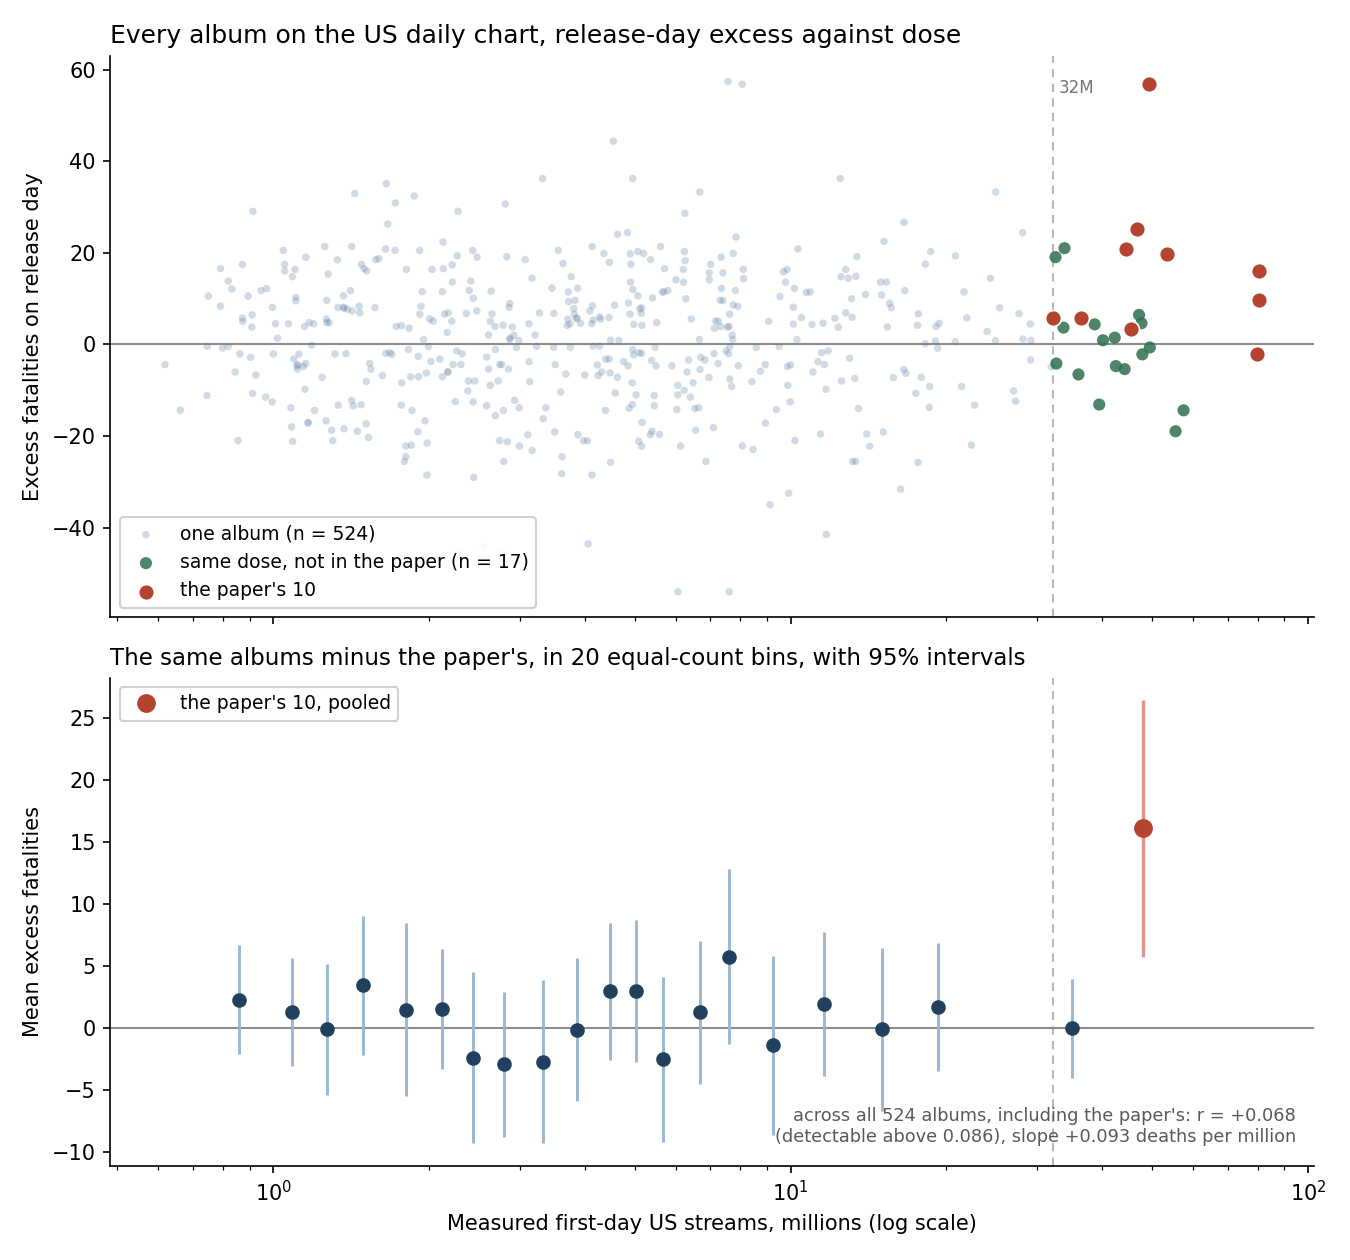
\includegraphics[width=\textwidth]{../figs/dose_response.png}
\caption{Release-day excess fatalities against measured first-day US streams, for every
album on the daily Spotify top 200 between 2017 and 2024 with at least three charting
tracks released on the same day and a fatality residual available ($n = \numNDoseAll$).
Excess is the residual from the donut model of Section~\ref{sec:replication}: observed
release-day fatalities minus the prediction of a day-of-week, month, year and holiday
model fitted with release windows excluded. The dashed line marks $\numDoseCut$ million
streams, the smallest of the ten albums in \citet{patel2026smartphones}; red points are
those ten and green points are the $\numNDoseMatched$ other albums that reach the same
dose. The lower panel drops the paper's ten and groups the rest into twenty equal-count
bins on the same logarithmic axis, with bin means and 95\% intervals from the spread of
albums within a bin; the red point is the paper's ten pooled, plotted at their median
dose. The horizontal line is zero excess.}
\label{fig:dose}
\end{figure}

\begin{table}
\caption{Release-day excess by decile of measured first-day US streams, across every album on the chart. The ten-album version of this test could not detect a correlation below 0.63; this one detects above 0.086.}
\begin{tabular}{rrrrr}
\toprule
dose\_bin & n & dose\_median & effect\_mean & effect\_se \\
\midrule
0 & 53 & 0.971 & 2.112 & 1.576 \\
1 & 52 & 1.401 & 2.466 & 2.061 \\
2 & 52 & 1.958 & 0.395 & 2.007 \\
3 & 53 & 2.688 & -3.441 & 2.299 \\
4 & 52 & 3.734 & -0.680 & 2.054 \\
5 & 52 & 4.927 & 2.422 & 2.089 \\
6 & 53 & 6.399 & 0.872 & 2.146 \\
7 & 52 & 8.663 & 1.864 & 2.598 \\
8 & 52 & 13.747 & -0.718 & 2.185 \\
9 & 53 & 32.096 & 4.538 & 1.891 \\
\bottomrule
\end{tabular}
\end{table}


\subsection{A Frame Anyone Can Rebuild}

Ranking every album released between 2018 and 2022 by measured first-day US streams
replaces a hand-assembled list with a rule. The estimate is present at every frame size
and declines monotonically as the frame widens, from $+\numEffectFrameTen$ on the top ten
to $+\numEffectFrameFifty$ on the top fifty.

\begin{table}
\caption{Albums 2018-2022 ranked by measured first-day US streams from Spotify Charts, so the sample is generated by a rule rather than assembled by hand. The estimate is present at every frame size and falls as the frame widens.}
\begin{tabular}{rrrrrrrr}
\toprule
frame\_size & n\_albums & min\_first\_day\_millions & effect & se & ci\_lower & ci\_upper & p\_value \\
\midrule
10 & 10 & 45.408 & 13.242 & 5.688 & 0.374 & 26.110 & 0.045 \\
15 & 15 & 36.341 & 10.078 & 4.254 & 0.953 & 19.203 & 0.033 \\
20 & 20 & 31.912 & 7.248 & 3.405 & 0.122 & 14.373 & 0.047 \\
30 & 30 & 21.908 & 6.361 & 2.843 & 0.547 & 12.176 & 0.033 \\
50 & 50 & 15.539 & 4.313 & 2.055 & 0.183 & 8.443 & 0.041 \\
\bottomrule
\end{tabular}
\end{table}


That decline is what selection on the largest releases looks like when it is measured
rather than argued. The effect is real at every cut, and its magnitude is largest where
the sample is most extreme, which is the same conclusion the out-of-sample albums reached
by a different route.

\section{Limitations of This Critique}
\label{sec:limits}

Weather enters through daily precipitation from NOAA GHCN stations in all fifty states and the
District of Columbia, aggregated with fixed weights equal to each state's share of US traffic
fatalities from 2007 to 2024, so the control weights by where fatal crashes happen and nothing in
it is a function of the crash record. Adding it moves the estimate from \numEffectNoWeather{} to
\numEffectWeatherControlled{}, a spread of \numWeatherSpread{} deaths across weightings.

\input{../tabs/t43_exogenous_weather}

That series has three limits. One station per state under-represents weather inside large states.
It covers precipitation only: GHCN precipitation includes the water equivalent of snow, but
snowfall as a separate variable is absent, because GSOD carries snow depth rather than snowfall
amount. And five states use their principal airport rather than a downtown station, since downtown
co-operative records are too sporadic.

The weather variables that appear in the crash-composition tables are shares of the fatal crashes
that occurred in rain, fog, cloud or snow, computed from the crash file itself. Numerator and
denominator are both the outcome, so the share falls mechanically when release days add crashes,
which makes them inadmissible as controls \citep{angrist2009mostly}. They are reported as
description of what the extra crashes looked like and nothing conditions on them.

The measured dose is censored from below. The chart covers the top two hundred songs, so an album
contributes only its charting tracks and an album that places three tracks is measured less
completely than one that places twenty. The censoring applies to \citet{patel2026smartphones}
equally, since its streaming series is the same product. It also bounds coverage in time: the US
daily chart begins in 2017, so the \numNAllAlbums{}-album panel still rests on a hand-assembled
list for earlier releases, and the reproducible frame of Section~\ref{sec:streaming} runs from
2018 forward.

The alcohol decomposition splits crashes on a characteristic the release itself may change. It
locates the excess and cannot identify what produced it, and no comparison built from the crash
record alone can, because the crash record does not say who was listening to anything.

With ten treated units in the original sample and \numNAllAlbums{} in the broader panel, all
inference here is fragile, and that cuts both ways. The out-of-sample estimate has an interval
that touches zero. The 2023--2024 subset that looks like a break rests on seven albums.
Small-sample instability affects this critique exactly as it affects the paper. The
dose-matched contrast is the one comparison here that does not depend on a small treated group
for its comparison side, and its \numNDoseMatched{} comparison albums are still few enough that
its interval spans five deaths in each direction.

\section{Conclusion}

The anomaly on the original ten dates is real, it replicates closely, and it is not an artifact of
the day of the week. Random Fridays do not reproduce it, the comparison is invariant to whether
weekday dummies are in the model, letting Friday vary by season and by year leaves it intact, a
model-free contrast against each album's own neighbouring Fridays recovers it, and the calendar
positions carry nothing in other years. The day $-6$ coefficient that looks like a pre-trend is a
Saturday, and the actual previous Friday is flat.

What does not hold is the size. Ten treated days cannot detect an effect below \numMDEEighty{}
deaths, and at the paper's own standard error the threshold exceeds the estimate it reports.
Outside the ten chosen dates the pooled effect is $+\numEffectOutsidePaper$ with an interval that
touches zero, and a true effect of that size, filtered through significance, produces published
estimates averaging \numMeanPublishedAtOutside{}. The anomaly on those ten dates is real; the
effect of releasing an album is much smaller than the number attached to it.

Measuring the dose sharpens that from an interval to a comparison. The
\numNDoseMatched{} albums whose first day on the US chart was at least as large as the paper's
smallest release show no release-day excess at all, \numEffectDoseMatched{} deaths against
$+\numEffectResidual$ for the ten. Whatever produced the anomaly, it was not the size of the
release.

The mechanism is a separate question and remains open. The comparison that most directly supports
distraction covers all ten albums, but it splits crashes on a characteristic
the release itself may change, so it describes where the excess sits and cannot say why. The rival
explanation that would matter most, ambient activity, is answerable with public data and does not
hold.

The broader lesson is not about music. Narrow-window designs built on a handful of salient dates
have produced striking estimates before, on election days \citep{zhang2016election} and on the
cannabis holiday \citep{palayew2019cannabis, brown2018reexamining}, and the reanalyses have tended
to find smaller effects rather than none. A design that can only see large effects will only ever
report large ones. The remedy is more treated units, and here they were sitting in the same data
product the original paper used to measure its treatment.

\bibliographystyle{plainnat}
\bibliography{ms}

\end{document}